\documentclass[10pt]{article}
\usepackage[utf8]{inputenc}
\usepackage[T1]{fontenc}
\usepackage{amsmath}
\usepackage{amsfonts}
\usepackage{amssymb}
\usepackage{mhchem}
\usepackage{stmaryrd}
\usepackage{graphicx}
\usepackage[export]{adjustbox}
\graphicspath{ {./images/} }

\title{Optimization of Optical Receiver Parameters for Pulsed Laser Tracking Systems }


\author{Zarko P. Barbaric [\^{}1], Lazo M. Manojlovic [\^{}2]}
\date{}


\begin{document}
\maketitle
Microwave Review



\begin{abstract}
An analysis of the reception of optical signals on the position sensitive optical receiver is presented in this paper. The optical receiver and electronics for analog signal processing measure the angle displacements between the optical axis of the receiver and the direction optical receiver - designated object, based on current signals, which are generated on the avalanche quadrant photodiode. Special attention was paid to the transipmedance preamplifier and the atmospheric turbulence as the key factors which limit the long range in pulsed laser tracking systems.
\end{abstract}

Keywords - Position sensitive optical receiver, pulsed laser \(\begin{array}{lllll}\text { tracking } & \text { systems, } & \text { avalanche } & \text { quadrant } & \text { photodiode, }\end{array}\) transimpedance amplifier, atmospheric turbulence.

\section{INTRODUCTION}
Today's usage of the pulsed laser systems is very wide in the field of civil and maritime engineering as well as for the military purpose [1]. By using a pulsed laser designator and the corresponding optical receiver some parameters of the laser illuminated object can be determined, such as the distance to the object and its angle displacements. The principle of distance and angle displacements measurements is based on the laser pulses emission, which illuminates the object, whose parameters are to be determined, and their reception with the corresponding optoelectronic receiver [2]. After the analog signal processing, the above mentioned parameters can be determined. By controlling the dynamic range of the received reflected optical radiation and using a well-designed analog signal processing chain, it is possible to reach the accuracy of several millimeters in measuring the distances of several hundreds of meters. To measure the angle displacements it is necessary to use, instead of a standard photodiode, the optical receiver, whose response depends on the light spot position on its surface. There are several types of such an optical receiver, but the quadrant photodiode and the lateral effect photodiode are the most common [3]. The quadrant photodiode is almost exclusively used in pulsed laser tracking systems because of its increased sensitivity and lower

Zarko P. Barbaric is with Electrotechnical Faculty, University of Belgrade, Bulevar kralja Aleksandra 73, 11000 Belgrade, Serbia and Montenegro, E-mail: barbaric@etf.bg.ac.yu

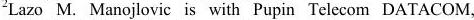
\includegraphics[max width=\textwidth]{d2750892714501b765cfde22b041f38a-01} Batajnicki put 23, 11080 Belgrade, Serbia and Montenegro, E-mail: lazom \((\) apupintelecom.co.yu overall noise compared to the lateral effect photodiode. Recently, the avalanche quadrant photodiode with a good matching of each segment avalanche amplification can be found on the market. The advantage in using avalanche quadrant photodiode is in the lower overall noise compared to standard quadrant P-i-N photodiode.

The basic subject of this paper is the optimization of the receiver parameters for pulsed laser tracking systems. The reflected optical radiation from the illuminated object is collected on the receiving optics. The received optical power levels, from the object and the background mostly determine the characteristics of the pulsed laser tracking system. Therefore, the estimations of the received optical powers are given in Part 0 . The position sensitive optical detector consists of both the receiving optics and the analog signal processing chain, used for processing signals from the quadrant photodiode. A more detailed description of a position sensitive optical receiver is given in Part 0 .

The most significant part of an analog signal processing is the preamplifier. As an optimal solution for the preamplifier the transimpedance amplifier is used. In Part 0 the optimal transimpedance configuration for achieving the minimal overall noise in the receiving chain is presented. The equivalent input noise current was calculated as the optimal avalanche amplification of each avalanche photodiode.

Part 0 shows how the atmospheric turbulence influences the measurement precision. The angle-of-arrival fluctuations and illumination fluctuations were taken into consideration. Finally, in Part 0 the total measurement error was calculated and the optimal receiver parameters for achieving the maximal positioning and tracking range for pulsed laser tracking systems was found.

\section{RECEIVED OPTICAL POWERS}
For determining the maximum range of the positioning and tracking of objects illuminated by pulsed laser, it is necessary first of all to find the levels of optical powers which we have at the position sensitive optical receiver (PSOR). It is well known that the error of angle measurement is strongly dependent on a signal-to-noise ratio at the output of a receiving chain. In further analysis, the geometrical parameters of the laser designator, illuminated object and of the optical receiver, which are shown on Fig. 1, will serve to find optical power levels at the input of the optical receiver.

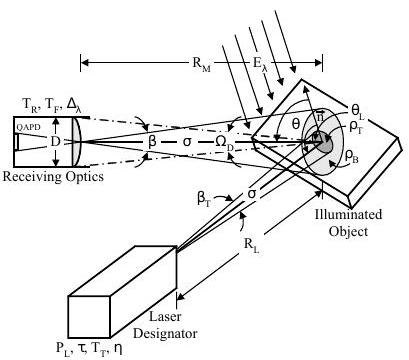
\includegraphics[max width=\textwidth]{d2750892714501b765cfde22b041f38a-02}

Fig. 1. Geometry of the laser transmitter and the receiving optics.

In the analysis, it is assumed, for the sake of generalization, that the laser designator and the receiving optics are located at different platforms, as it is presented on Fig. 1. Analysis of the optical power levels of a background and reflected laser designator optical signal is conducted on the basics of the well-known radiometrical equation [1]. For the background and the object, it is assumed to be diffuse reflectors which reflecting as a Lambertian source [1]. It is also assumed that the whole laser beam is falling on the surface of the illuminated object.

\section{A. Background Power}
The optical power of a background \(P_{B}\), which is received at the input of an PSOR, is [2]:
\[
P_{B}=L_{\lambda} G T_{R} T_{F} \tau_{a t}
\]
where \(L_{\lambda}\) is the solar spectral radiance at the object site, \(G\) is a geometrical factor, \(T_{R}\) is the receiving optics transmission coefficient, \(T_{F}\) is the optical filter transmission coefficient, \(\tau_{t}\) is the transmission coefficient of the atmosphere. The geometrical factor \(G\) is defined as a factor of radiation exchange of two small areas:
\[
G=\frac{A_{D} \cos \theta \cdot A_{R} \cos \theta_{p o}}{R_{M}^{2}}
\]
where \(A_{D}\) is the area of the detector footprint at the background, \(A_{R} \cos \theta_{p o}\) is the effective area of the optical receiver, \(\theta\) is the angle between object surface normal and the line joining the object and receiver centers, \(\theta_{p o}\) is the angle between the receiver surface normal and the line joining the object and receiver centers \(\left(\theta_{p o}=0\right.\), because in the case of good positioning and tracking the receiving optics is always directed towards the object) and \(R_{M}\) is the distance between the object and the optical receiver.

The solar spectral radiance \(L_{\lambda}\), induced by solar radiation of a diffuse reflector for a specific wavelength \(\lambda\) is given as \([1]:\)
\[
L_{\lambda}=\frac{E_{\lambda} \rho_{B}}{\pi}
\]
where \(E_{\lambda}\) is the solar spectral irradiance and \(\rho_{B}\) is the background reflectance.

The atmosphere transmittion coefficient \(\tau_{u t}\) is given as:
\[
\tau_{a t}=e^{-\sigma R_{M}}
\]
where \(\sigma\) is the atmospheric extinction coefficient.

The background power, which is given in Eq. (1), after combining with Eqs. (2) to (4), becomes:
\[
P_{B}=\frac{\pi}{16} E_{\lambda} \Delta_{\lambda} \rho_{B} \beta^{2} D^{2} T_{R} T_{F} e^{-\sigma R_{\mu}}
\]
where \(\Delta_{\lambda}\) is the optical spectral filter bandwidth, \(\beta\) is the receiving optics field-of-view, \(D\) is the receiving optics aperture diameter.

\section{B. Signal Power}
The received optical signal power \(P_{S}\), of the reflected laser radiation from the illuminated object, in the case when the area of the laser beam is smaller than the area of the object, is equal to [1-2]:
\[
P_{S}=L_{T} A_{T} \Omega_{D} T_{R} T_{F} e^{-\sigma R_{\omega}} \cos \theta
\]
where \(L_{T}\) is the spectral radiance of the reflected radiation from the object, \(A_{T}\) is the area of the laser spot on the object, \(\Omega_{D}\) is the solid angle subtended by the optical receiver aperture. The spectral radiance \(L_{T}\) is:
\[
L_{T}=\frac{4 P_{L} T_{T} \eta \rho_{T} e^{-\sigma R_{t}} \cos \theta_{L}}{\pi^{2} \beta_{T}^{2} R_{L}^{2}}
\]
where \(P_{L}\) is the laser peek power, \(T_{T}\) is the transmission coefficient of transmitting optics, \(\eta\) is the transmitting optics collection efficiency, \(\rho_{T}\) is the target reflectance, \(\theta_{L}\) is the angle between the object surface normal and the laser beam, \(\beta_{T}\) is the laser beam divergence angle and \(R_{L}\) is the distance between the laser and the object.

For the surface \(A_{T}\) of the laser spot on the object the following is valid:
\[
A_{T}=\frac{\pi R_{l}^{2} \beta_{T}^{2}}{4 \cos \theta_{L}}
\]
and for the solid angle \(\Omega_{D}\) :
\[
\Omega_{D} \approx \frac{\Pi D^{2}}{4 R_{M}^{2}}
\]
Combining Eqs. (7) to (9) with Eq. (6), we finally obtain the following for the received signal optical power \(P_{S}\) :
\[
P_{S}=\frac{D^{2}}{4 R_{M}^{2}} P_{L} \rho_{T} T_{T} \eta T_{R} T_{F} e^{-\sigma\left(R_{L}+R_{\mu}\right)} \cos \theta
\]

\section{THE POSITION SENSITIVE OPTICAL RECEIVER}
In this paragraph the principles of the angles of azimuth and elevation measurement using the PSOR and the avalanche quadrant photodiode (AQPD) in pulsed laser tracking systems will be explained. Fig. 2 gives the arrangement of the key optical elements and geometrical parameters of the AQPD in the PSOR.

Fig. 2. The PSOR and the AQPD.

The purpose of the optical receiver of the OEC, which is shown on Fig. 2 (a), is to collect the reflected optical energy from the illuminated object. The planoconvex lens, which is placed at the input of the optical receiver, collects the incoming optical energy on the AQPD. To minimize the error the planoconvex aspherical lens is mostly used, because of its minimal spherical aberration coefficient. By using such a lens the most uniform distribution of the irradiance on the AQPD is achieved. The AQPD is located behind the lens at the distance \(d\) from it. Fig. 2 (b) gives the example of AQPD located in front of focal plane, e.g. \(d<f\), where \(f\) is the focal length of the lens. As the AQPD isn't placed at the focal plane, a light spot with an approximately uniform distribution of irradiance is formed on its surface. The radius of the light spot is equal to \(r_{0}\). From the well known geometrical relations the following equation for the spot radius is obtained:
\[
r_{o}=\frac{D|f-d|}{2 f}
\]
where \(D\) is the diameter of the lens, \(f\) is the focal length and \(d\) is the distance between the lens and the AQPD.

In the case when the optical axis and the line objectreceiver are not collinear, the light reflected from the object comes with a relatively small angle inclination \(\varepsilon_{x}\) towards the optical axis. The center of a light spot formed in such a way is moved for the distance \(x\) regarding the center of the AQPD, as it is presented on Fig. 2 (b). As the angle \(\varepsilon\) is small \(\left(\varepsilon_{x} 1\right)\), then it is easy to show that the light spot radius doesn't change significantly with the light spot movement across the AQPD. Everything above mentioned is also valid for the second plane, i.e. for the angle \(\varepsilon_{y}\) and for the distance \(y\). Assuming that the reflected optical radiation is uniform, the uniform light spot on the AQPD is obtained, as it is resented on Fig. 2 ©. Two cases are shown on this figure. The first case is when the optical axis and the line object-receiver are collinear. In that case the light spot center is at the AQPD center. In the second case the optical axis and the line object-receiver are not collinear and then the light spot is moved regarding to the AQPD center where \(x\) and \(y\) are the displacements of the light spot along the \(x\) - and \(y\) -axis, respectively.

When the centers of the light spot and the AQPD are matched all four photodiodes are illuminated with the same amount of optical radiation, so all four photodiode currents are the same. In the case when the light spot center is moved, the optical power is divided into four different parts, so the currents of each photodiode are different. By processing these currents it is possible to obtain the estimation of the distances \(x\) and \(y\). On the basics of the determined distances it is possible to obtain the values of angle displacements \(\varepsilon_{x}\) and \(\varepsilon_{y}\) as:
\[
\varepsilon_{x}=\operatorname{arctg} \frac{x}{d} \approx \frac{x}{d}, \varepsilon_{y}=\operatorname{arctg} \frac{y}{d} \approx \frac{y}{d}
\]
As it can be seen from Eq. (12), angles \(\varepsilon_{x}\) and \(\varepsilon_{v}\) are in direct proportion to the displacements of light spot center \(x\) and \(y\), but only when the following relations are valid \(|x| d\) and \(|y| \quad d\).

One of the most important parameters of each PSOR is its field of view \(\beta\), for which \(\beta=2 \operatorname{arctg}(r / d) \approx 2 r / d\) is valid, where \(r\) is the AQPD radius. The maximal range of measured angles \(\left(\varepsilon_{x, y}\right)_{\max }\), which can be measured with such an PSOR is equal to: \(\left|\varepsilon_{x, y}\right|_{\max }=\beta / 2 \approx r / d\). According to this, by the designing of geometrical parameters of the PSOR it is needed to pay the special attention should be paid to defining the minimal allowed value of the receiver field of view under which the system for positioning and tracking can function correctly. Otherwise, in certain situations the PSOR can lose the object, which can be critical especially in systems such as laser guided missiles.

\section{A. Light Spot Displacement Measurement}
Direct measurements of displacements \(x\) and \(y\) by processing signals from the AQPD isn't possible. By measuring the signals it is possible to determine the ratios of displacements and light spot radius, e.g. \(x / r_{0}\) and \(y / r_{0} .\) For determining these relations it is essential to know the irradiance distribution on the AQPD surface. Here it is assumed for the distribution to be uniform.

The exact measurements of the ratios \(x / r_{0}\) and \(y / r_{0}\) aren't possible and only the estimations can be made with the following equations [3-5]:

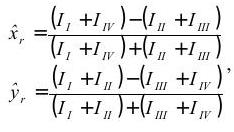
\includegraphics[max width=\textwidth]{d2750892714501b765cfde22b041f38a-03}

Septembar 2003 .

where \(\hat{x}_{r}\) and \(\hat{y}_{r}\) are the estimated values of the ratios \(x / r_{0}\) and \(y / r_{0}\), respectively and \(I_{I}, I_{I}, I_{I I I}\) and \(I_{I V}\), are the AQPD peek currents. For these currents \(I_{K}=M R_{k} P_{K}\) is valid, where \(M\) is the avalanche photodiode amplification, \(R_{K}\) is the photodiode conversion factor and \(P_{K}\) are the AQPD peek optical powers \((K=I\), II, III and \(I V\) ). Finally from Eq. (13) the following is obtained for the \(x\) -axis:
\[
\left.\hat{x}_{r}=\frac{\left(P_{I}+P_{I V}\right)-\left(P_{I I}+P_{I I I}\right)}{\left(P_{I}+P_{I V}\right)+\left(P_{I I}+P_{I I}\right.}\right)
\]
If the irradiance on the AQPD surface is uniform then for the AQPD powers the following can be stated: \(P_{K}=E_{0} S_{K}\) where \(E_{0}\) is the irradiance at the AQPD surface and \(S_{K}\) is the area of the illuminated part of the \(K\) -th quadrant of the AQPD. Taking that into consideration, we can write [5]:
\[
\left.\hat{x}_{r}=\frac{\left(S_{I}+S_{I V}\right)-\left(S_{I I}+S_{I I I}\right)}{\left(S_{I}+S_{I V}\right)+\left(S_{I I}+S_{I I}\right.}\right)
\]
This is the most common case in pulsed laser tracking systems.

Now it is important to find the range of the displacements \(x\) and \(y\) for which the whole light spot is located at the AQPD. This will provide a good linear dependence of \(x\) and \(y\) and the measured values at the output of the AQPD. The whole light spot is on the \(\mathrm{AQPD}\) if the following relation is fulfilled: \(\sqrt{x^{2}+y^{2}}+r_{o} \leq r\). This inequality yields to \(|x| \leq r_{0}\) and \(|y| \leq-r_{0}\). For the angle range on the basis of Eq. (12) the following is valid: \(\left|\varepsilon_{x}\right| \leq\left(r-r_{0}\right) / d\) and \(\left|\varepsilon_{y}\right| \leq\left(r-r_{0}\right) / d\). According to the angle range requirements, the parameters of the AQPD such as the light spot radius \(r_{0}\) and the distance between AQPD and the lens \(d\) should be determined. Wishing to provide a good linearity all four photodiodes must be illuminated. This is fulfilled if \(|x| \leq_{0}\) and \(|y| \leq_{0}\). On the basis of these inequalities, the optimal value of the light spot radius is obtained when both of these two inequalities are fulfilled at the same time, and this is when the following is satisfied: \(r_{0}=r-r_{0}\). This yields to optimal light spot radius to be \(r_{0}=r / 2\).

To find the relations between the light spot displacements and the measured values it is necessary to determine the illuminated areas of the AQPD \(S_{K}\) where \(K=I, I I\), III and \(I V\). For these areas, from Fig. 3 , it can be written:
\[
\begin{array}{l}
S_{I}+S_{I V}=r_{0}^{2} \pi-\left(S_{I I}+S_{I I I}\right) \\
S_{I I}+S_{I I}=r_{0}^{2} \pi \frac{\alpha}{2 \pi}-\frac{1}{2} L x
\end{array}
\]
where \(\alpha\) and \(L\) are the geometrical values which are shown on Fig. 3. For angle \(\alpha\) the following is valid: \(\alpha=2 \arccos \left(x / r_{0}\right)\) and for length \(L\) : \(L=2 r_{0} \sin (\alpha / 2)\). By substituting the last two equation in Eq. (16) the following equations is obtained:
\[
S_{I I}+S_{I I I}=r_{0}^{2}\left[\arccos \left(\frac{x}{r_{0}}\right)-\frac{x}{r_{0}} \sqrt{1-\left(\frac{x}{r_{0}}\right)^{2}}\right]
\]
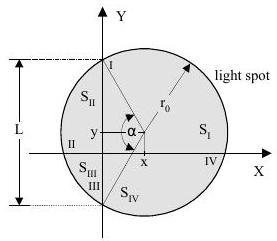
\includegraphics[max width=\textwidth]{d2750892714501b765cfde22b041f38a-04}

Fig. 3. Geometry of the light spot on the AQPD.

Combining Eqs. (15) to (17) finally we have for \(\hat{x}_{r}\) the following:
\[
\hat{x}_{r}=1-\frac{2}{\pi}\left[\arccos \left(\frac{x}{r_{0}}\right)-\frac{x}{r_{0}} \sqrt{1-\left(\frac{x}{r_{0}}\right)^{2}}\right]
\]
If we assume that the displacements are small values in regard to the light spot radius, i.e. \(x r_{0}\), we have:
\[
\hat{x}_{r} \approx \frac{4}{\pi} \frac{x}{r_{o}}=S_{Q P D} x
\]
where \(S_{Q P D}\) is the AQPD incremental sensitivity. In the case of the irradiance uniform distribution: \(S_{Q P D}=4 / \pi_{0}\).

On the basis of Eq. (19) we can obtain the estimated value of the light spot displacement \(\hat{x}\), for which we can write:
\[
\hat{x}=\frac{\pi}{4} r_{0} \hat{x}_{r}=K_{Q P D} \hat{x}_{r}
\]
where \(K_{Q P D}=1 / S_{Q P D}=\pi_{0} / 4\) is the proportional factor between the measured and the estimated values of the light spot displacements. As it can be seen from Eq. (19) the incremental sensitivity is in an inverse proportion to the light spot radius, which means that the minimal light spot radius is needed for the maximum sensitivity.

\section{B. Noise Induced Measurement Error}
Noise, which is inherent to any electronic device, is one of the most significant causes of the angle measurement error in pulsed laser tracking systems. According to Eq. (13) and taking into consideration the equivalent noise sources, we can write:
\[
\left.\hat{x}_{r}=\frac{\left(I_{I}+I_{n I}+I_{I V}+I_{n V}\right)-\left(I_{I I}+I_{n I I}+I_{I I I}+I_{n I I I}\right)}{\left(I_{I}+I_{n I}+I_{I V}+I_{n V}\right)+\left(I_{I I}+I_{n I I}+I_{I I I}+I_{n ! I I}\right.}\right)
\]
where \(I_{n i}\) is the equivalent noise current of \(i\) -th photodiode. If we adopt \(U=I_{l}+I_{I V}\) and \(V=I_{I I}+I_{I I I}\) and \(U_{n}=I_{n l}+I_{n I V}\) and \(V_{n}=I_{n I I}+I_{n I I I}\), we will obtain:
\[
\hat{x}_{r}=\frac{\left(U+U_{n}\right)-\left(V+V_{n}\right)}{\left(U+U_{n}\right)+\left(V+V_{n}\right)} \text { . }
\]
If we rearrange the Eq. (22) and assuming that \(U_{n}+V_{n} U+V\) we will get:
\[
\hat{x}_{r} \approx \frac{U-V}{U+V}+2 \frac{V U_{n}-U V_{n}}{(U+V)^{2}}
\]
The first part of Eq. (23) represents the mean value of the relative light spot displacement and the second part represents the random error in displacement measuring caused by noise. For this measurement error \(\hat{x}_{r n}\) we can write:
\[
\hat{x}_{r n} \approx \frac{2 V}{(U+V)^{2}} U_{n}-\frac{2 U}{(U+V)^{2}} V_{n} .
\]
As the noise sources in each receiving channel are independent, for the variance \(\sigma_{\dot{x},}^{2}\) of the relative displacement measurement the following is valid:
\[
\sigma_{\hat{x}_{r}}^{2} \approx \frac{4 V^{2}}{(U+V)^{4}} \sigma_{u}^{2}+\frac{4 U^{2}}{(U+V)^{4}} \sigma_{v}^{2}
\]
where \(\sigma_{u}^{2}\) and \(\sigma_{v}^{2}\) are the variances of the \(U_{n}\) and \(V_{n}\), respectively and \(\sigma_{u}^{2}=\sigma_{v}^{2}=2 \overline{i_{n}^{2}}\), where \(\overline{i_{n}^{2}}\) is the variance of the noise current in each receiving channel. Now, Eq. (25) can be rearranged in:
\[
\sigma_{\dot{x}_{r}}^{2} \approx 8 \frac{U^{2}+V^{2}}{(U+V)^{4}} \bar{i}_{n}^{2}
\]
As for \(U\) and \(V, S_{S}=U+V\) is valid, where \(S_{s}\) is the signal in the summing channel, the variance \(\sigma_{\hat{x}}^{2}\) of the relative displacement measurement becomes:
\[
\sigma_{\hat{x}_{r}}^{2} \approx 8 \frac{U^{2}+\left(S_{S}-U\right)^{2}}{S_{S}^{4}} \overline{i_{n}^{2}}
\]
The variance \(\sigma_{\hat{x}_{2}}^{2}\), from Eq. (27), has the minimum value for \(U=S_{S} / 2\) and \(V=S_{S} / 2\), so we can write:
\[
\left(\sigma_{\hat{x}_{,}}^{2}\right)_{\min } \approx \frac{4 \overline{i_{n}^{2}}}{S_{S}^{2}}=\frac{1}{S N R_{\Sigma}}
\]
where \(S N R_{\Sigma}\) is signal-to-noise ratio in summing channel. As it can be seen, the minimal variance of the relative displacement measurement is achieved when \(U=V=S_{S} / 2\) is valid, i.e. when the light spot center is at the AQPD center. According to Eq. (20), for the minimal value of the estimated light spot displacement standard deviation \(\left(\sigma_{\dot{x}}\right)_{\min }\) we have:
\[
\left(\sigma_{\dot{x}}\right)_{\min } \approx \frac{\pi}{4} \frac{r_{0}}{\sqrt{S N R_{\Sigma}}}
\]
The identical expression is valid for the standard deviation \(\left(\sigma_{\hat{y}}\right)_{\min }\) of the estimated displacement along the y-axis. On the basics of Eqs. (12) and (29) for the minimal standard deviation \(\left|\sigma_{\varepsilon_{\varepsilon}}\right|_{\min }\) of measured angle, in the case of uniform irradiance distribution, we have:
\[
\left(\sigma_{\varepsilon_{x}}\right)_{\min } \approx \frac{\pi}{4} \frac{r_{o}}{d} \frac{1}{\sqrt{S N R_{\Sigma}}}
\]
The parameters \(U\) and \(V\) are satisfy the following inequalities: \(U S S_{S}\) and \(V \leq S_{S} .\) Because of that and according to Eq. (27), the maximal value of the \(\left(\sigma_{\dot{x}}\right)_{\max }\) is achieved when \(U=S_{S}\) and \(V=0\) (or \(V=S_{S}\) and \(U=0\) ) is fulfilled, i.e. when the light spot center is at the measurement span margin \(\left(x=\pm r_{0}\right.\) and/or \(y=\pm r_{0}\) ), so we have:
\[
\left(\sigma_{\dot{x}}^{2}\right)_{\max } \approx \frac{2}{S N R_{\Sigma}}
\]
Identically, for the maximal standard deviation of estimated displacement along the \(\mathrm{x}\) -axis \(\left(\sigma_{\dot{x}}\right)_{\max }\) and the measured angle \(\left(\sigma_{\varepsilon_{s}}\right)_{\max }\), are valid:
\[
\begin{array}{l}
\left(\sigma_{\hat{x}}\right)_{\max } \approx \frac{\pi \sqrt{2}}{4} \frac{r_{0}}{\sqrt{S N R_{\Sigma}}} \text { and } \\
\left(\sigma_{\varepsilon_{s}}\right)_{\max } \approx \frac{\pi \sqrt{2}}{4} \frac{r_{0}}{d} \frac{1}{\sqrt{S N R_{\Sigma}}}
\end{array}
\]
The identical expressions are valid for the maximal standard deviation of estimated displacement along the \(\mathrm{y}\) -axis \(\left(\sigma_{\hat{y}}\right)_{\max }\) and the measured angle \(\left|\sigma_{\varepsilon_{y}}\right|_{\max } .\) As it can be seen, the maximal standard deviation of measured displacements and angles are \(\sqrt{2}\) times bigger than their minimal values, which doesn't represent a significant enlargement. For us of interest is the minimal error in positioning and tracking, because in the case when the centers of the light spot and the AQPD are matched, we have a good positioning and tracking.

The required span of the measured angles depends on the dynamics of the pulsed laser tracking system. This measurement span is determined by the receiving optics fieldof-view \(\beta\). The receiving optics is designed in such a way to cover, with its field-of-view, the complete range of measured angles. According to Eq. (30) and the relations between the field-of-view, the AQPD radius and the light spot radius, for the noise induced angle measurement error \(\sigma_{\varepsilon_{l}}\) we can write:
\[
\sigma_{\theta_{t}} \approx \frac{\pi}{16} \beta \frac{1}{\sqrt{S N R_{\Sigma}}}
\]
As it can be seen from Eq. (34), it is recommended to choose the value of field of view as minimal as possible to minimize the angle measurement error. On the basis of Eq. (11) and the relations between field-of-view and the remaining OEC parameters and if \(\beta \quad 1\) is satisfied, there is a relation between the AQPD radius and the receiving optics aperture diameter: \(r \approx \beta f_{n o} D / 2\), where \(f_{n o}\) is the f-number of the lens, for which \(f_{n o}=f / D\) is valid.

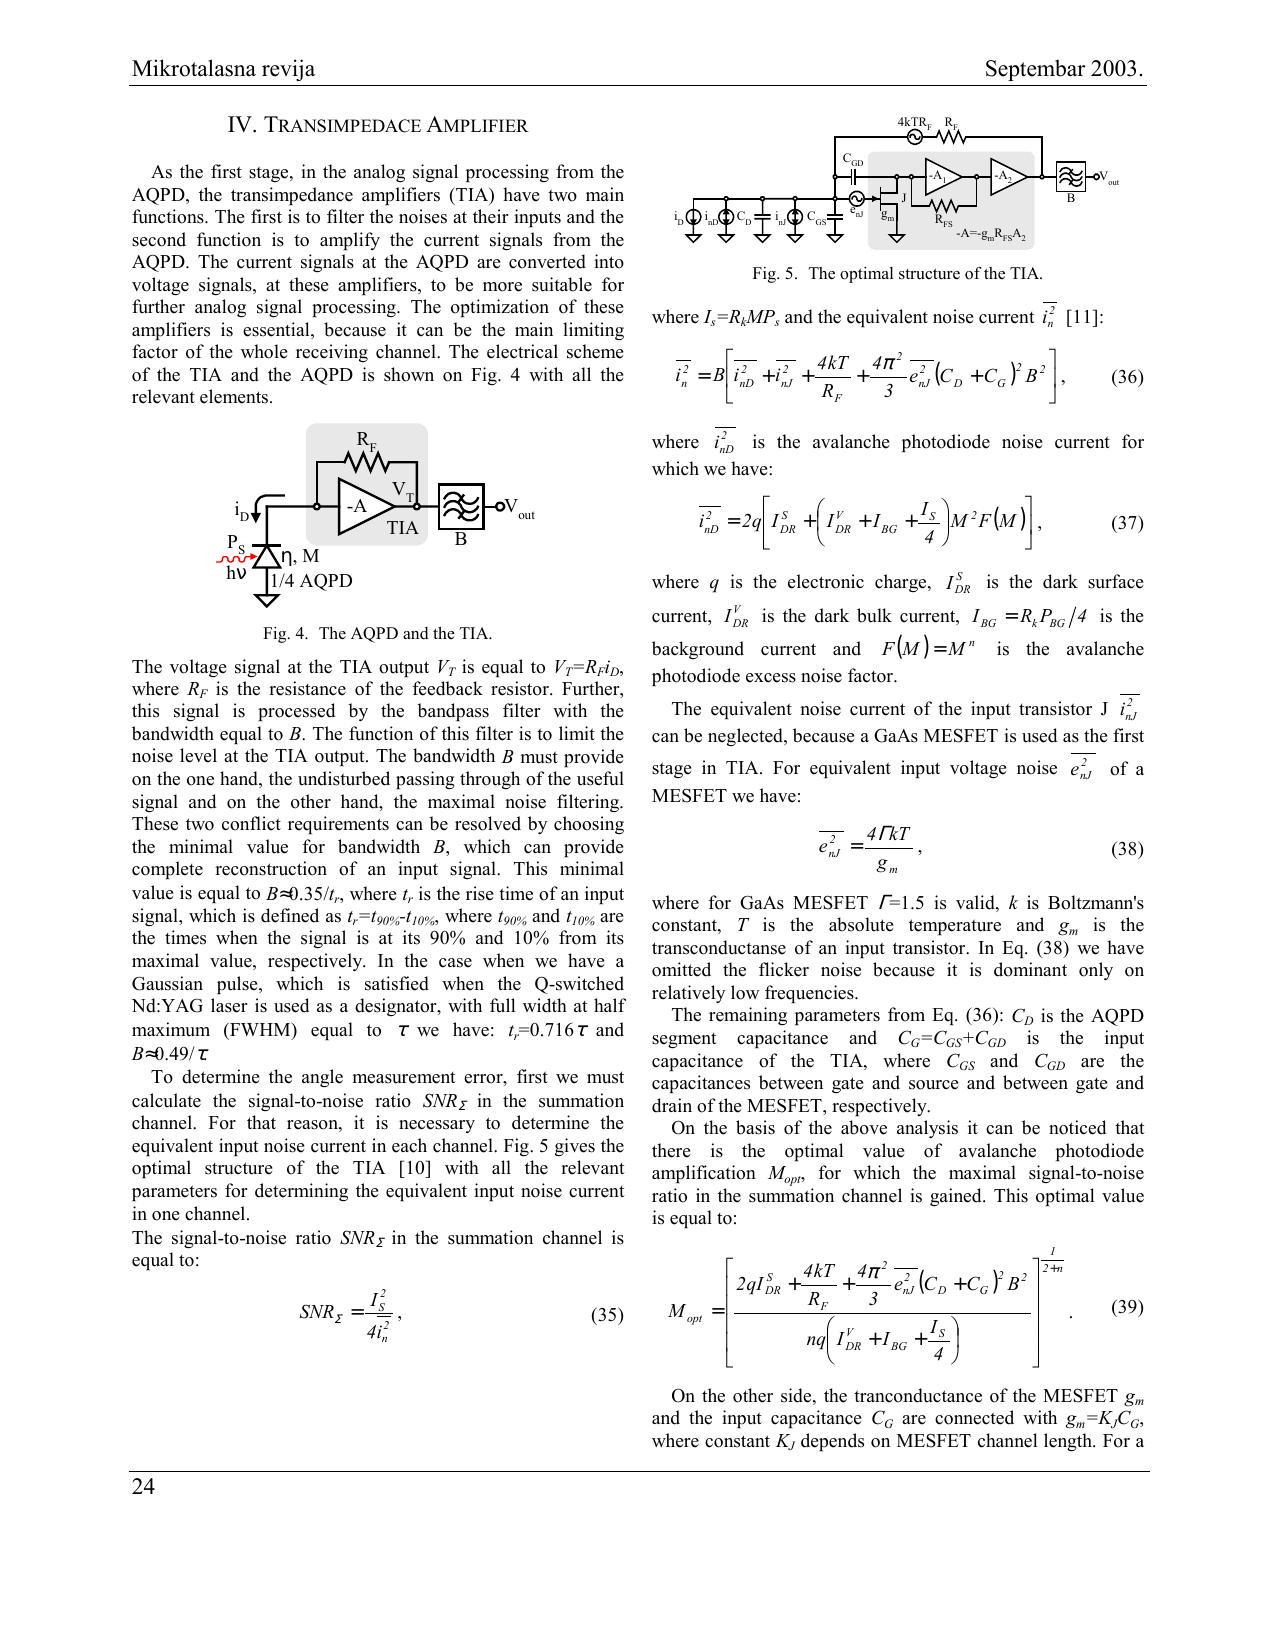
\includegraphics[max width=\textwidth]{d2750892714501b765cfde22b041f38a-06}

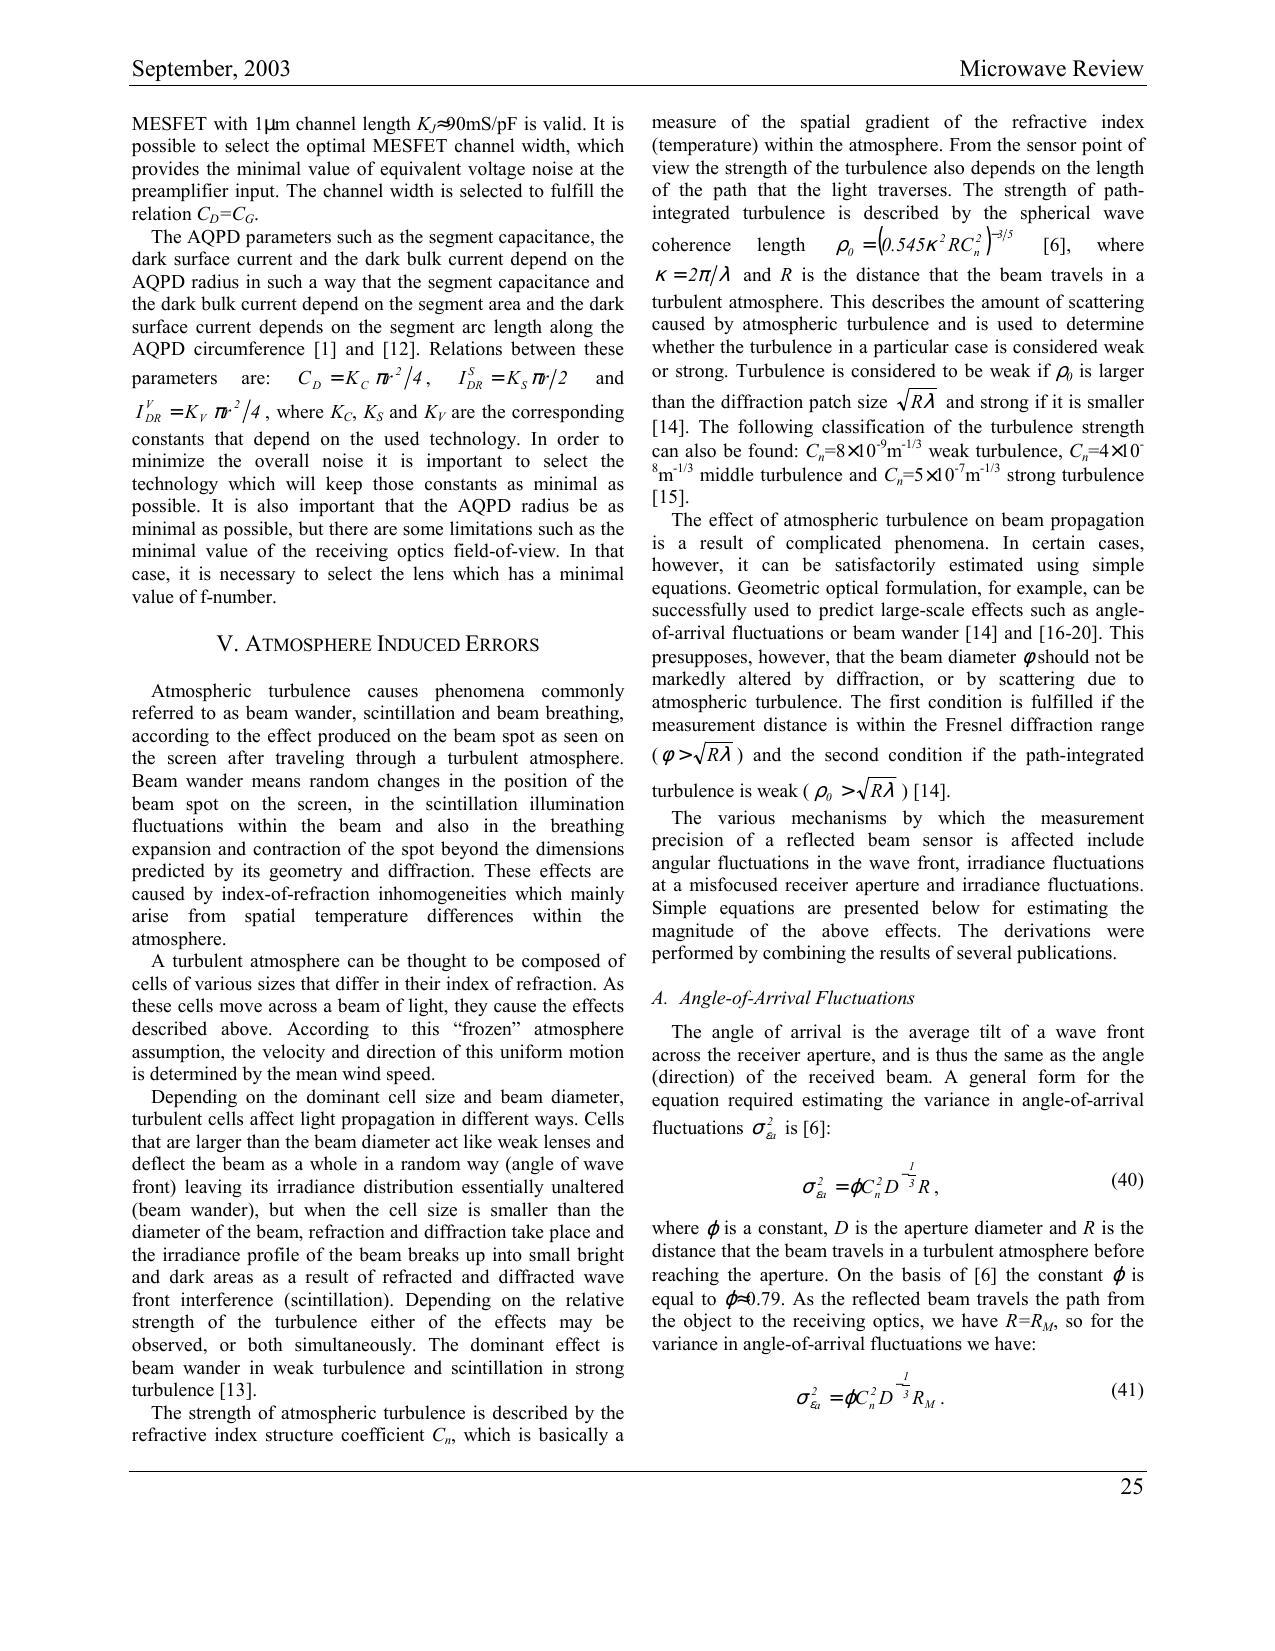
\includegraphics[max width=\textwidth]{d2750892714501b765cfde22b041f38a-07}

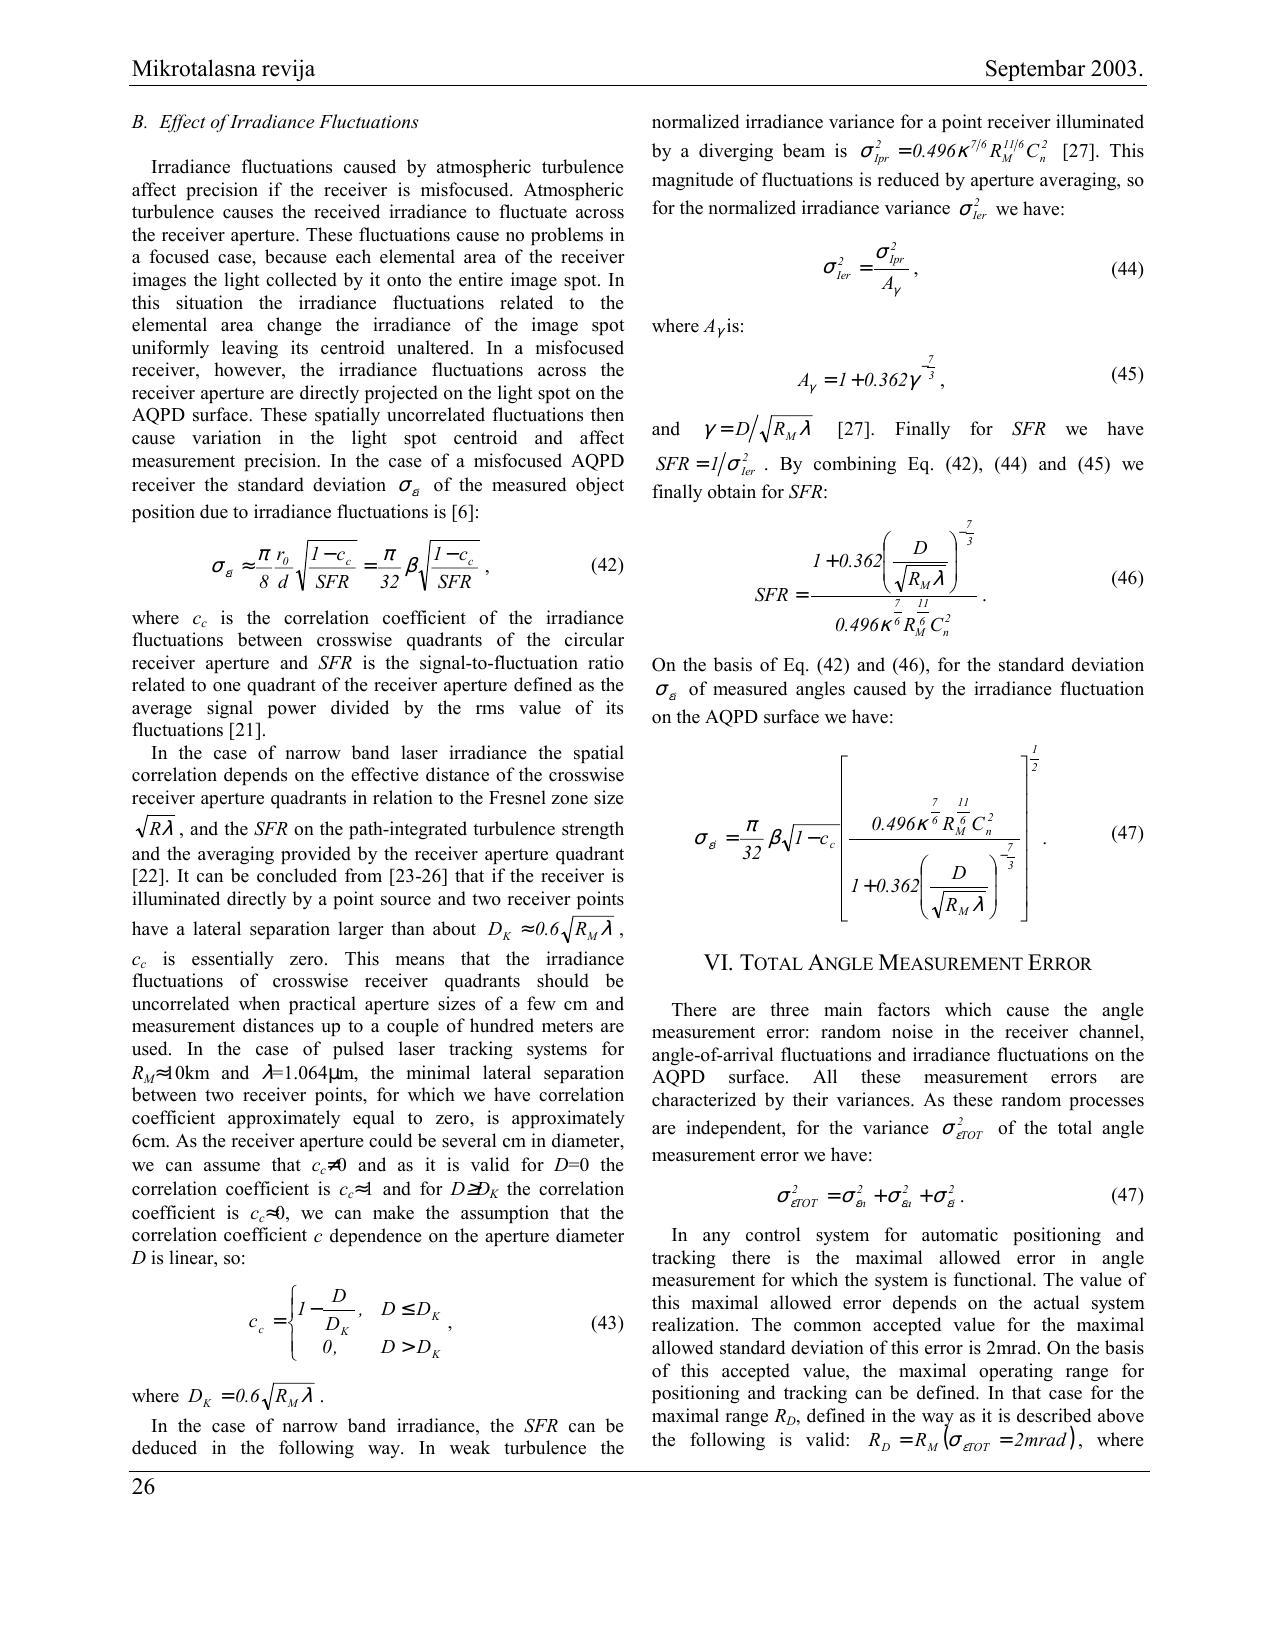
\includegraphics[max width=\textwidth]{d2750892714501b765cfde22b041f38a-08}

\(R_{M}\left(\sigma_{\varepsilon TOT}=2 \mathrm{mrad}\right)\) is the distance between the illuminated object and the receiver at which the total angle measurement error is equal \(2 \mathrm{mrad}\). On Fig. 6 the dependence between the maximal range \(R_{D}\) and the receiver aperture diameter \(D\) for the following parameters is presented: laser peak power \(P_{L}=5 \mathrm{MW}\), FWHM of the laser pulse \(\tau=20 \mathrm{~ns}\) (energy per laser pulse is approximately equal to \(\left.E_{L} \approx 00 \mathrm{~mJ}\right)\), field-of-view of the receiving optics \(\beta=10^{\circ}\), MESFET constant \(K_{5}=90 \mathrm{mS} / \mathrm{pF}\), MESFET excess noise factor \(\Gamma=1.5\), optical filter spectral bandwidth \(\Delta_{\lambda}=1 \mathrm{~nm}\), receiving optics transmission coefficient \(T_{R}=0.9\), optical filter transmission coefficient \(T_{F}=0.4\), refractive index structure coefficient \(C_{n}=8 \times 10^{-9} \mathrm{~m}^{-1 / 3}\) (this value for the refractive index structure coefficient is taken because it represents the mean value in the case of weak turbulence), avalanche photodiode excess noise factor coefficient \(n=0.4\), transimpedance resistance \(R_{F}=10 \mathrm{k} \Omega\), avalanche photodiode conversion coefficient for unit gain \(R_{k}=0.45 \mathrm{~A} / \mathrm{W}\), avalanche photodiode technology coefficients \(K_{C}=1 \mathrm{pF} / \mathrm{mm}^{2}, \quad K_{S}=3 \times 10^{-8} \mathrm{~A} / \mathrm{mm}, K_{V}=1 \times 10^{-10} \mathrm{~A} / \mathrm{mm}^{2}[28], \mathrm{f}-\) number of the aspheric planoconvex lens \(f_{n o}=0.7\), background reflectance \(\rho_{B}=0.4\), target reflectance \(\rho_{l}=0.2\), atmospheric extinction coefficient \(\sigma=0.15 \quad 1 / \mathrm{km}\), laser-object distance \(R_{L}=2 \mathrm{~km}\), angle between object surface normal and the line joining the object and receiver centers \(\theta=45^{\circ}\), transmission coefficient of transmitting optics \(T_{T}=0.9\), transmitting optics collection efficiency \(\eta=0.6\), absolute temperature \(T=300 \mathrm{~K}\) and for solar spectral irradiance three values were taken \(E_{\lambda}=50\), 300 and \(600 \mathrm{~W} /\left(\mathrm{m}^{2} \mu \mathrm{m}\right)\)

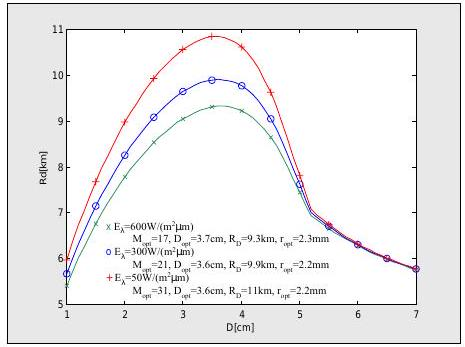
\includegraphics[max width=\textwidth]{d2750892714501b765cfde22b041f38a-09}

Fig. 6. The maximal range dependence on the aperture diameter.

As it can be seen from Fig. 6 there is an optimal value of the receiving optics aperture diameter \(D_{o p t}\) for which the pulsed laser tracking system has the maximal positioning and tracking range. Although we have changed the value of solar spectral irradiance in the wide range, the optimal value of the receiving optics aperture diameter has just slightly changed. The optimal value of this diameter is in the range of \(3.6 \mathrm{~cm}\) to \(3.7 \mathrm{~cm}\). The optimal avalanche photodiode amplification is also changed in the relatively narrow range from 17 to 31 . Concerning the optimal aperture diameter and the minimal allowed field-of-view, the optimal radius of he AQPD has, also, just slightly changed.

\section{CONCLUSION}
Concerning the maximal range of positioning and tracking in pulsed laser tracking systems the optimal parameters of an optical receiver was found. It was shown that there is an optimal receiving optics aperture diameter which is slightly changed by changing the solar irradiance conditions. The optimal diameter is approximately equal to \(3.6 \mathrm{~cm}\) for a standard set of parameters, as shown in Part 0 . This optimal diameter value is in good matching with the aerodynamical requirements for laser guided missiles. Also, the optimal value of the AQPD radius was found to be equal to approximately \(2.2 \mathrm{~mm}\). This yields to the maximal possible range to be equal approximately \(10 \mathrm{~km}\).

\section{ACKNOWLEDGEMENT}
We wish to acknowledge the encouragement and support of Professor A. Marincic.

\section{REFERENCES}
[1] H. N. Burns, C. G. Christodoulou, G. D. Boerman, ,System Design of a Pulsed Laser Rangefinders", Optical Engineering, Vol. 30, No. 3, pp 323-329, March 1991.

[2] Zarko Barbaric and Mirjana Nikolic, ,Parametrical Analysis of Pulsed Laser Rangefinder's Range", XLII ETRAN Conference Proceedings, Vrnjacka Banja, \(3-5\) Jun \(1998 .\)

[3] W. L. Wolfe and G. J. Zissis, The Infrared Handbook", Ann Arbor, Environmental Research Institute of Michigan, 1978 .

[4] Ernest O. Doebelin, Measurement Systems Application and Design, Mc Graw-Hill, \(1990 .\)

[5] Leonid G. Kazovsky, , Theory of Tracking Accuracy of Laser Systems", Optical Engineering, Vol. 22, No. 3, pp 339-347, May/June \(1983 .\)

[6] Anssi Mäkynen, Position-Sensitive Devices and Sensor Systems for Optical Tracking and Displacement Sensing Applications, Academic Dissertation, University of Oulu, Department of Electrical Engineering, Oulu, 2000 .

[7] A. Mäkynen, J. Kostamovaara and R. Myllylä, ,Positioning Resolution of the Position-Sensitive Detectors in High Background Illumination", \(\quad\) IEEE \(\quad\) Transactions \(\quad\) on Instrumentation and Measurement, Vol. 45, No. 1, pp 324-326, \(1996 .\)

[8] Y. Yanhai, , The Design of Echo Spot and Optical Focusing in Automatic Laser Tracking", Optics and Laser Technology, Vol. 18, No. 2, pp 75-79, 1986 .

[9] P. W. Young, L. M. German and R. Nelson, ,Pointing, Acquisition and Tracking Subsystems for Space-Based Laser Communications", Proceedings of SPIE 616, pp \(118-128\), \(1986 .\)

[10] J. L. Hullett and S. Moustakas, , Optimum Transimpedance Broadband Optical Preamplifier Design", Optical and Quantum Electronics, 13, pp \(65-69,1981\).

[11] Lazo M. Manojlovic, Analysis and Optimization in Receiving Optical Signal from Optoelectronic Coordinator in Pulsed Laser Tracking Systems, Master Thesis, Electrotechnical Faculty, University of Belgrade, Belgrade, \(2003 .\)

[12] Hiroaki Ando, Hiroshi Kanbe, Tatsuya Kimura, Toyoshi Yamaoka and Takao Kaneda, ,"Characteristics of Germanium Avalanche Photodiodes in the Wavelength Region of \(1-1.6 \mu \mathrm{m}^{\prime \prime}\), IEEE Journal of Quantum Electronics, Vol. QE-14, No. 11, pp \(804-809,1978 .\) Septembar 2003 .

[13] H. Weichel, ,Laser Beam Propagation in the Atmosphere", SPIE, Bellingham, Washington, USA, pp 45-66, 1990 .

[14] J. H. Churnside and R. J. Lataitis, Statistics of a Reflected Beam in the Turbulent Atmosphere (Path Correlation), NOAA Technical Memorandum ERL WPL-172, National Oceanic and Atmospheric \(\quad\) Administration, \(\quad\) Environmental \(\quad\) Research Laboratories, Wave Propagation Laboratory, Boulder, Colorado, USA, 1989 .

[15] %Ж. Госсорг, Инфракрасная термография - Основы, механика, применение, Мир, Москва, \(1988 .\)

[16] R. S. Lawrence and J. W. Strohbehn, , A Survey of Clear-Air Propagation Effects Relevant to Optical Communications", Proceedings of the IEEE, Vol. 58, No. 10, pp \(1523-1545,1970\).

[17] T. Chiba, ,spot Dancing of the Laser Beam Propagated Through the Turbulent Atmosphere", Applied Optics, Vol. 10 , No. 11, pp 2456-2461, 1971.

[18] J. W. Dowling and P. M. Livingston, , Behavior of Focused Beams in Atmospheric Turbulence: \(\quad\) Measurements and Comments on the Theory", Journal of the Optical Society of America, Vol. 63, No. 7, pp 846-858, 1973 .

\(\begin{array}{lllllll}19 & \text { J. } & \text { H. Churnside and R. J. Lataitis, }, \text { , Angle-of-Arrival }\end{array}\) Fluctuations of a Reflected Beam in Atmospheric Turbulence", Journal of Optical Society of America \(A\), Vol. 4, No. 7, pp \(1264-1272,1987 .\)

[20] J. H. Churnside and R. J. Lataitis, , Wander of an Optical Beam in the Turbulent Atmosphere \(^{6 *}\), Applied Optics, Vol. 29, No. 7, pp \(926-930,1990\). [21] G. A. Andreev and R. M. Magind, Influence of Intensity Fluctuations on the Measurement of Angular Position of Radiation Source by Optical-Electron Monopulse Method, Izvestiya Vysshikh Uchebnykh Zavedenii Radiofizika, Vol. 15, No. 1, pp \(55-61,1972 .\)

[22] A. Mäkynen, J. Kostamovaara and R. Myllylä, ,Displacement \(\begin{array}{lll}\text { Sensing } & \text { Resolution of } \text { Position-Sensitive } & \text { Detectors in }\end{array}\) Atmospheric Turbulence Using Retroreflected Beam", IEEE Transactions on Instrumentation and Measurement, Vol. 46, No. 5, pp \(1133-1136,1997 .\)

[23] R. S. Lawrence and J. W. Strohbehn, , A Survey of Clear-Air Propagation Effects Relevant to Optical Communications", Proceedings of the IEEE, Vol. 58, No. 10, pp 1523-1545, 1970 . [24] R. L. Fante, , Electromagnetic Beam Propagation in Turbulent Media", Proceedings of the IEEE, Vol. 63, No. 12, pp 1669 \(1692,1975 .\)

\([25] \mathrm{W} .\) A. Coles and \(\mathrm{R}\). G. Frechlich, ,Simultaneous Measurement of Angular Scattering and Intensity Scintillation in the Atmosphere \(^{\prime \text { , }}\), Journal of Optical Society of America, Vol. 72, No. 8, pp \(1042-1048,1982 .\)

[26] J. H. Churnside and J. J. Wilson, , Enhanced Backscatter of a Reflected Beam in Atmospheric Turbulence", Applied Optics, Vol. 32, No. 15, pp \(2651-2655,1993\).

[27] H. Weichel, , Laser Beam Propagation in the Atmosphere", SPIE, Bellingham, Washington, USA: \(45-66,1990 .\)

[28] P. E. Webb, R. J. McIntyre, and J. Conardi, Properties of Avalanche Photodiodes, Technical Report, RCA, \(1977 .\)


\end{document}